
\subsection{Unveiling Good Sparse Solutions without Training}
In this section we show an strange phenomenon that we detect on convolutional networks.  
We add Gaussian noise to our pretrained network with a set global noise level
(standard deviation) $\sigma$ followed by standard Magnitude Pruning \cite{hanLearningBothWeights2015a,hanDeepCompressionCompressing2016a}. 
\begin{figure}
    \centering
    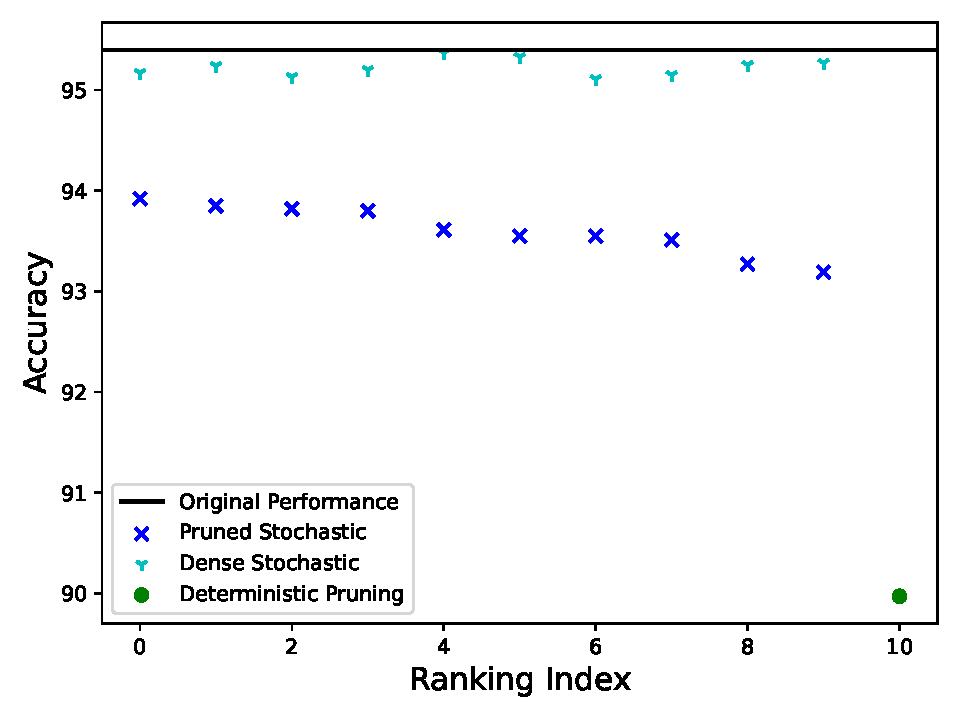
\includegraphics[width=0.45\textwidth]{figures/stochastic_deterministic_gaussian_sigma_0.002_pr_0.8_batchSize_512_pop_10_t_11-44_test.pdf}
    \caption{ Accuracy of one-shot pruned ResNet18 with 80\% sparsity in the CIFAR10 test set with $\sigma = 0.002$. In this case, 10 noisy samples were retrieved. Note that all dense noisy ResNet18 networks do not outperform the noiseless 
    original solution}
    \label{fig:stochastic_versus_deterministic}
\end{figure}

\begin{table}[!htb]
    \centering
    \caption{Median of weight magnitude per layer}
    \begin{tabular}{|l|l|}
    \hline
        \textbf{Layer Name} & \textbf{Median} \\ \hline
        conv1 & 5.29E-06 \\ \hline
        layer1.0.conv1 & 3.99E-07 \\ \hline
        layer1.0.conv2 & 5.41E-03 \\ \hline
        layer1.1.conv1 & 4.85E-03 \\ \hline
        layer1.1.conv2 & 4.24E-03 \\ \hline
        layer2.0.conv1 & 7.91E-03 \\ \hline
        layer2.0.conv2 & 7.53E-03 \\ \hline
        layer2.0.shortcut.0 & 1.17E-02 \\ \hline
        layer2.1.conv1 & 4.71E-03 \\ \hline
        layer2.1.conv2 & 4.39E-03 \\ \hline
        layer3.0.conv1 & 7.37E-03 \\ \hline
        layer3.0.conv2 & 6.74E-03 \\ \hline
        layer3.0.shortcut.0 & 9.55E-03 \\ \hline
        layer3.1.conv1 & 5.59E-03 \\ \hline
        layer3.1.conv2 & 4.07E-03 \\ \hline
        layer4.0.conv1 & 4.01E-03 \\ \hline
        layer4.0.conv2 & 2.24E-03 \\ \hline
        layer4.0.shortcut.0 & 4.41E-03 \\ \hline
        layer4.1.conv1 & 1.31E-03 \\ \hline
        layer4.1.conv2 & 7.08E-04 \\ \hline
        linear & 5.35E-02 \\ \hline
    \end{tabular}
    \label{tab:Q50perLayer}
\end{table}




% ####################################### Epsilon plotss##########################################
   
  % \begin{figure}[!htb]
  %   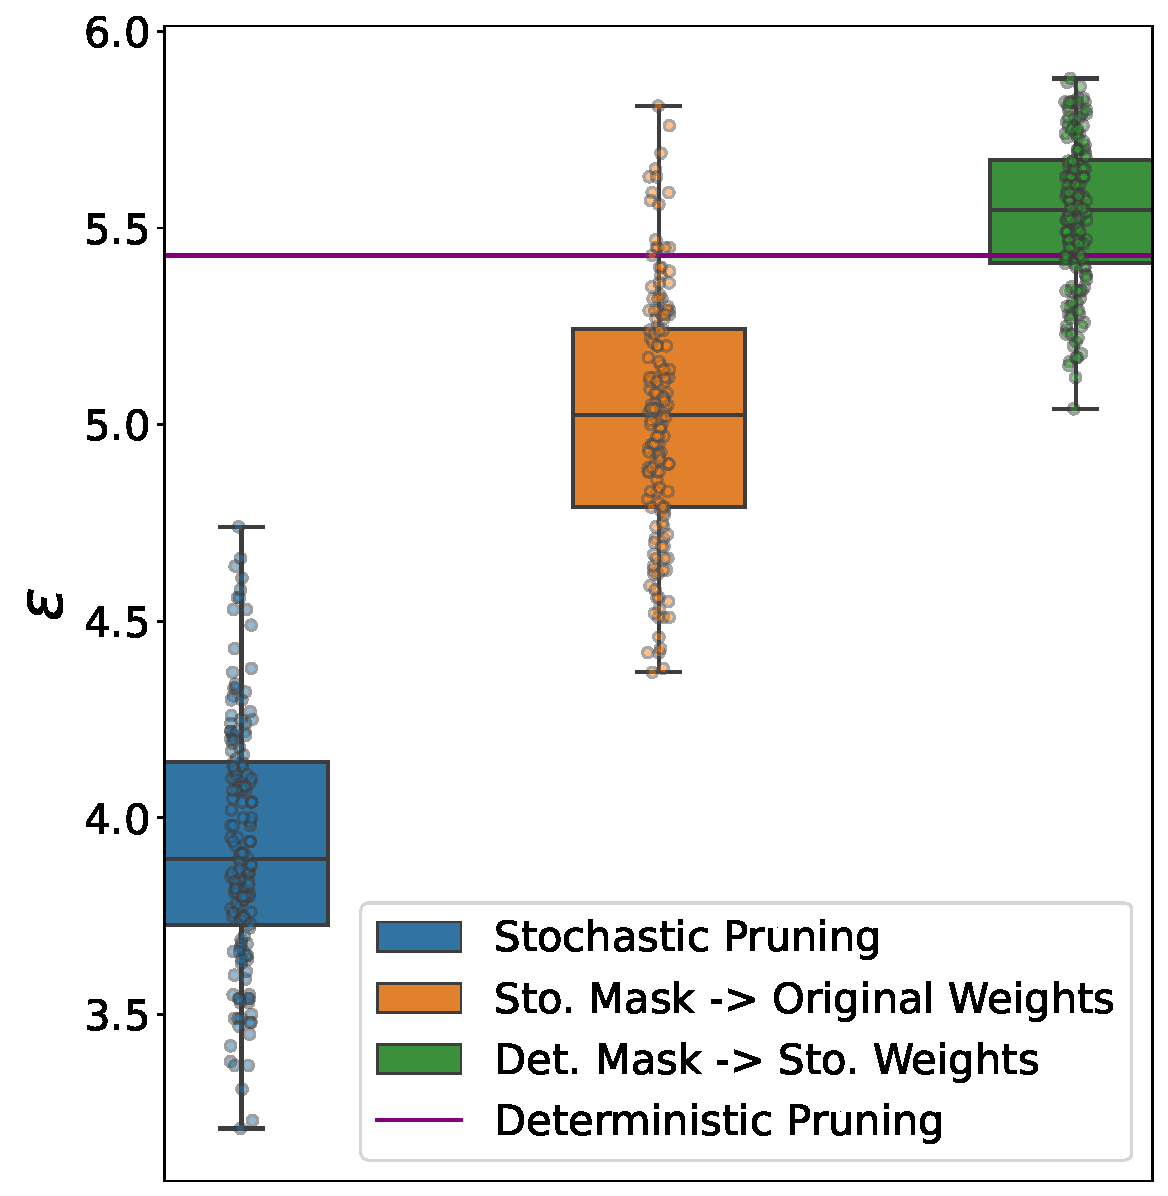
\includegraphics[width=\columnwidth]{figures/epsilon_allN_all_pr_0.8_sigma=0.001.pdf}
  %   \caption{Accuracy degradation of One-shot Stochastic Pruning with $\sigma=0.001$ and pruning rate of 0.8} \label{fig:pr0.8sigma0.001}
  % \end{figure}%
  % \begin{figure}[!htb]
  %   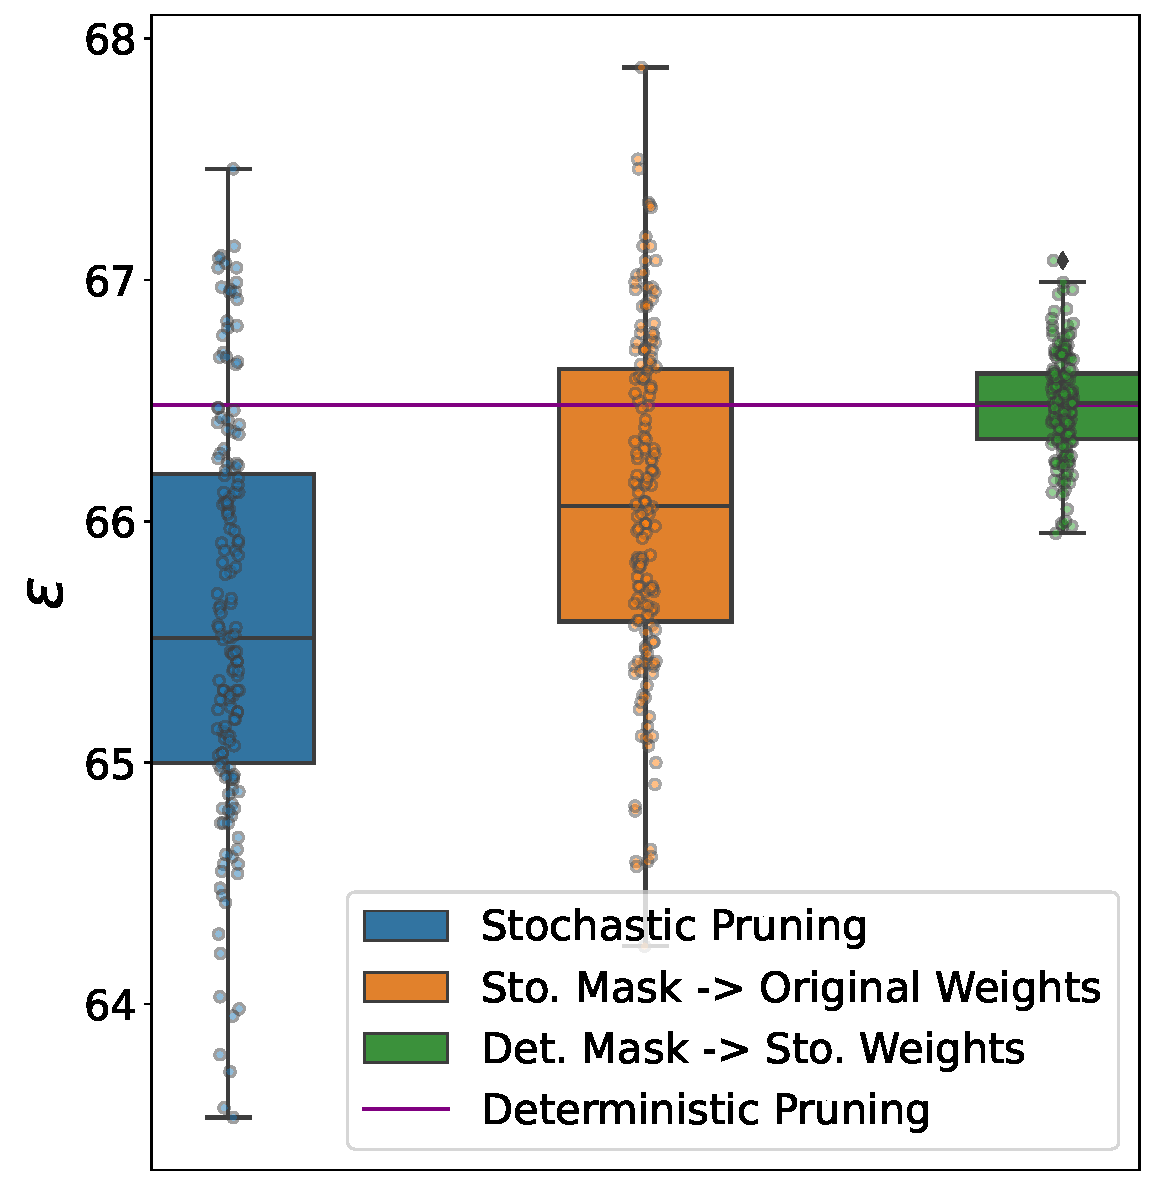
\includegraphics[width=\columnwidth]{figures/epsilon_allN_all_pr_0.9_sigma=0.001.pdf}
  %   \caption{Accuracy degradation of One-shot Stochastic Pruning with $\sigma=0.001$ and pruning rate of 0.9} \label{fig:pr0.9sigma0.001}
  % \end{figure}%



  % \begin{figure}[!htb]
  %   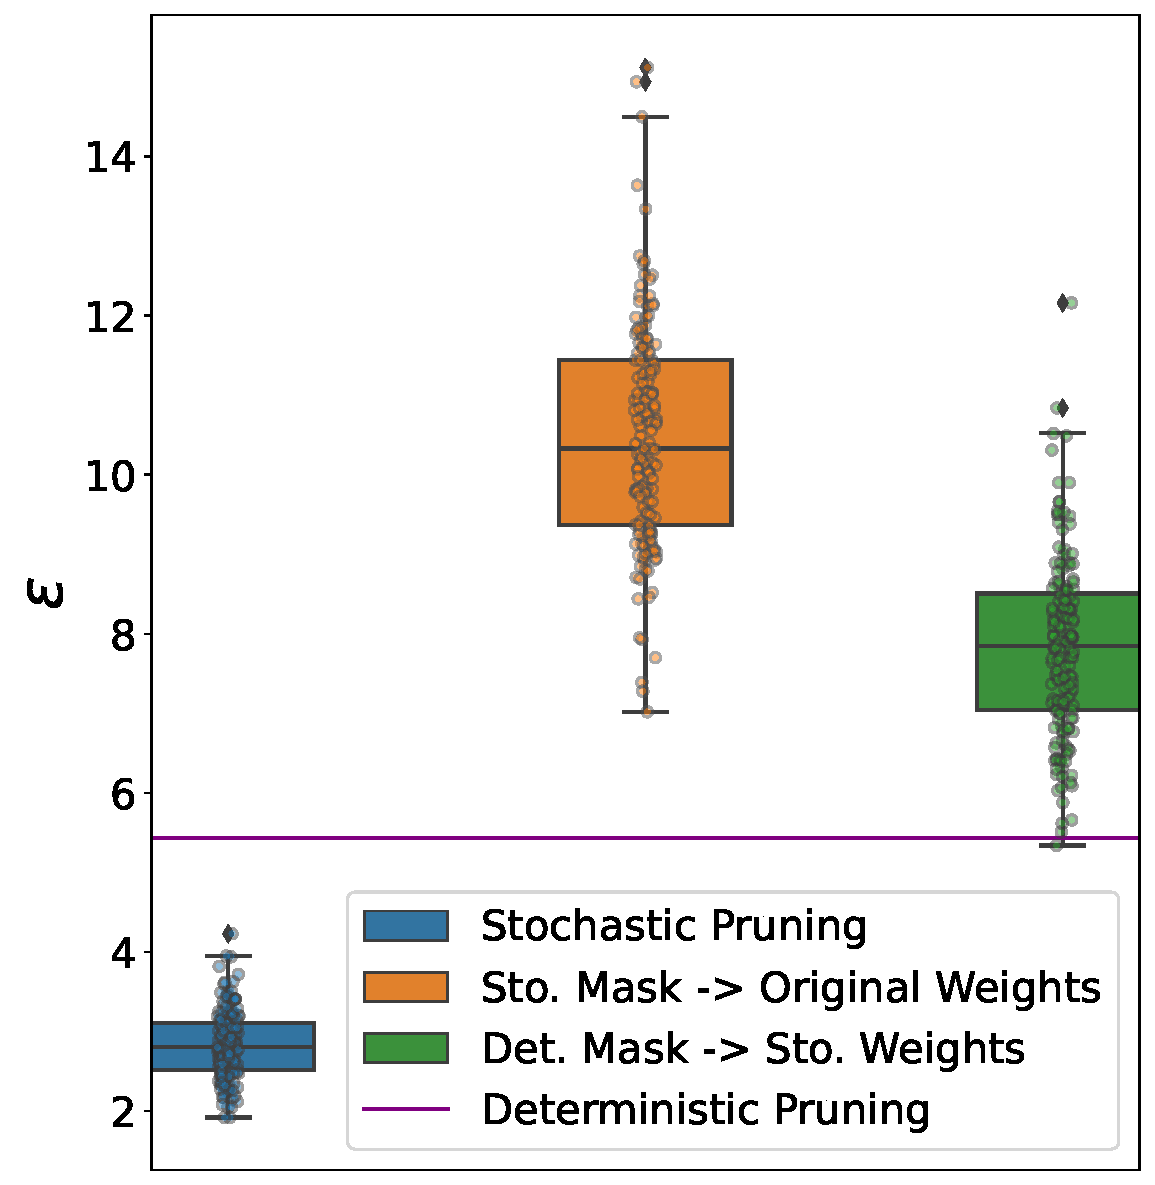
\includegraphics[width=\columnwidth]{figures/epsilon_allN_all_pr_0.8_sigma=0.005.pdf}
  %   \caption{Accuracy degradation of One-shot Stochastic Pruning with $\sigma=0.005$ and pruning rate of 0.8} \label{fig:pr0.8sigma0.005}
  % \end{figure}

  % \begin{figure}[!htb]
  %   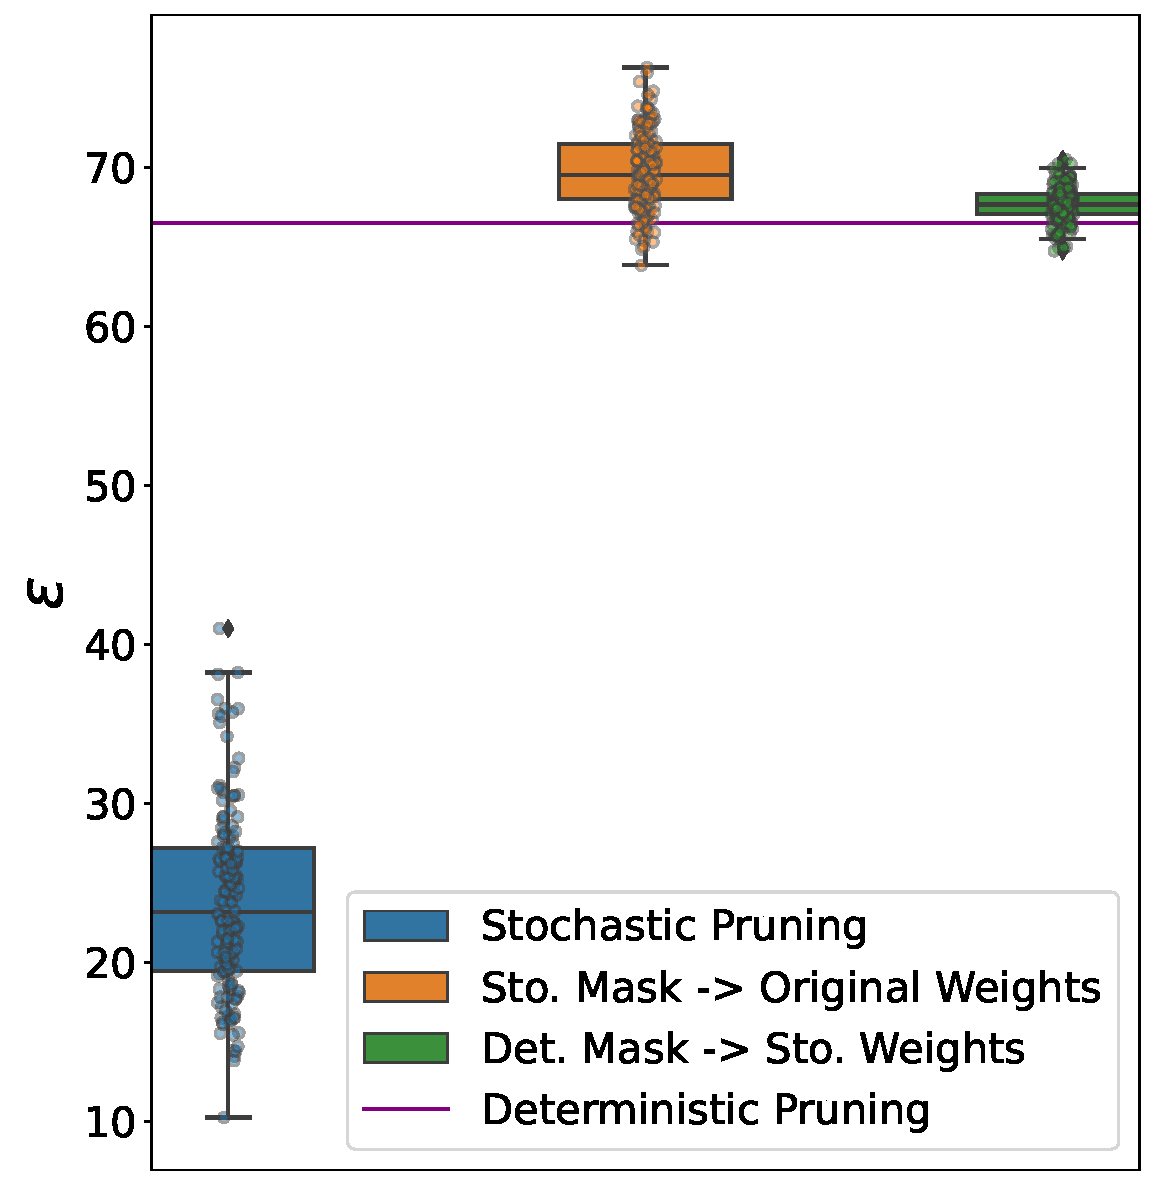
\includegraphics[width=\columnwidth]{figures/epsilon_allN_all_pr_0.9_sigma=0.005.pdf}
  %   \caption{Accuracy degradation of One-shot Stochastic Pruning with $\sigma=0.005$ and pruning rate of 0.9} \label{fig:pr0.9sigma0.005}
  % \end{figure}

\begin{figure*}[!htb]
  \centering
     \begin{subfigure}[b]{0.65\columnwidth}
         \centering
    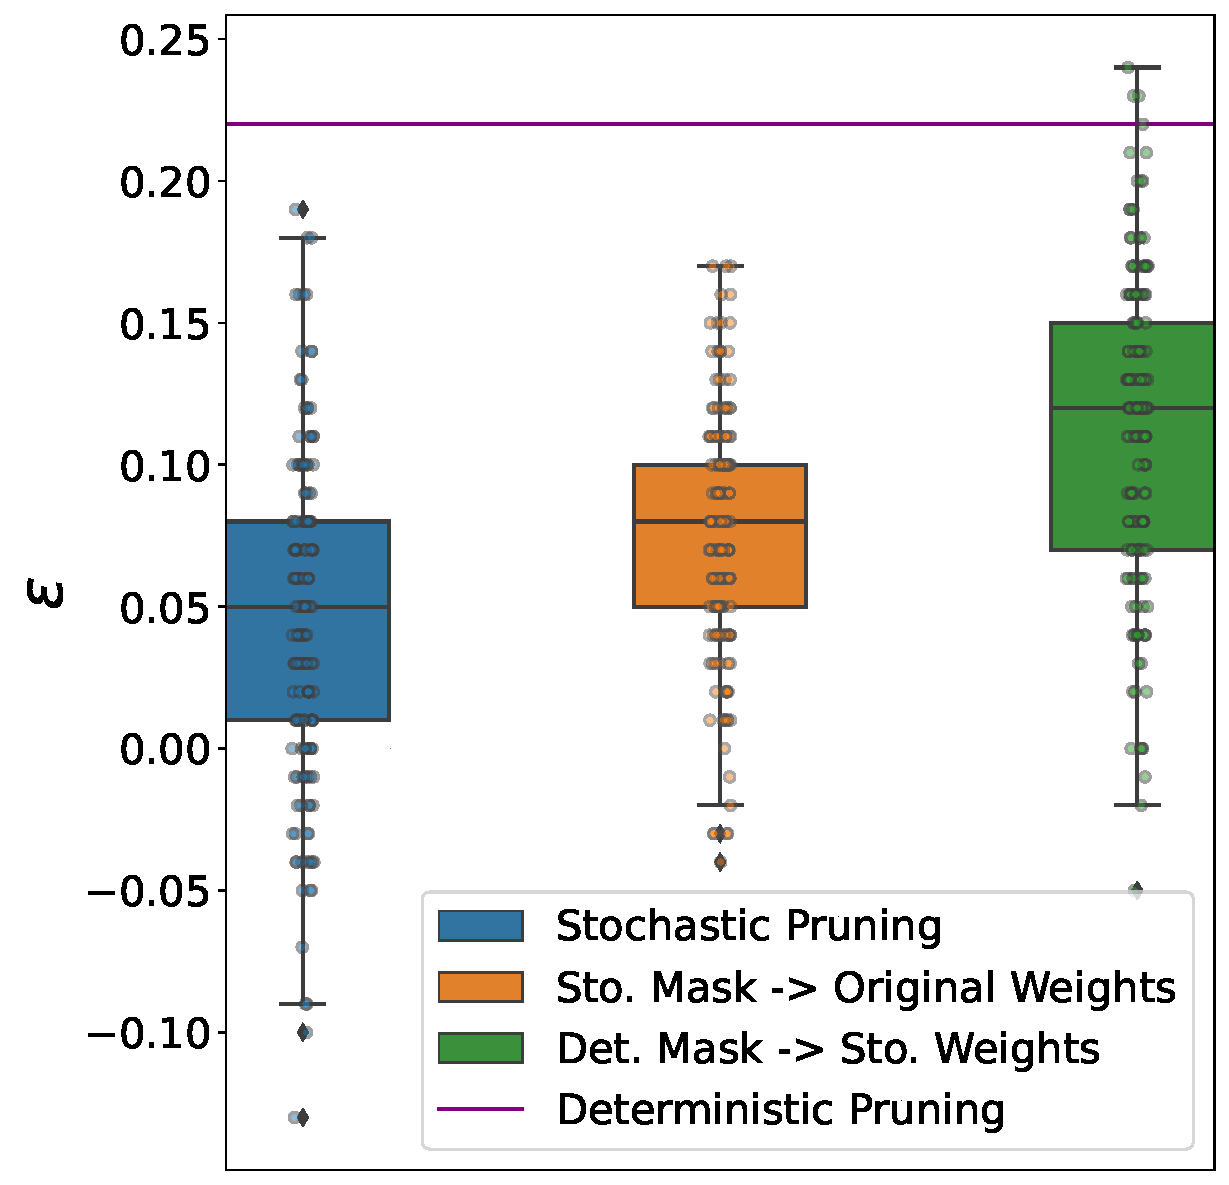
\includegraphics[width=\columnwidth]{figures/epsilon_allN_all_pr_0.5_sigma=0.001.pdf}
    % \caption{Accuracy degradation of One-shot Stochastic Pruning with $\sigma=0.001$ and pruning rate of 0.5} 
    \caption{ Pruning rate 0.5} 
    \label{fig:pr0.5sigma0.001}
     \end{subfigure}
     \hfill
     \begin{subfigure}[b]{0.65\columnwidth}
         \centering
   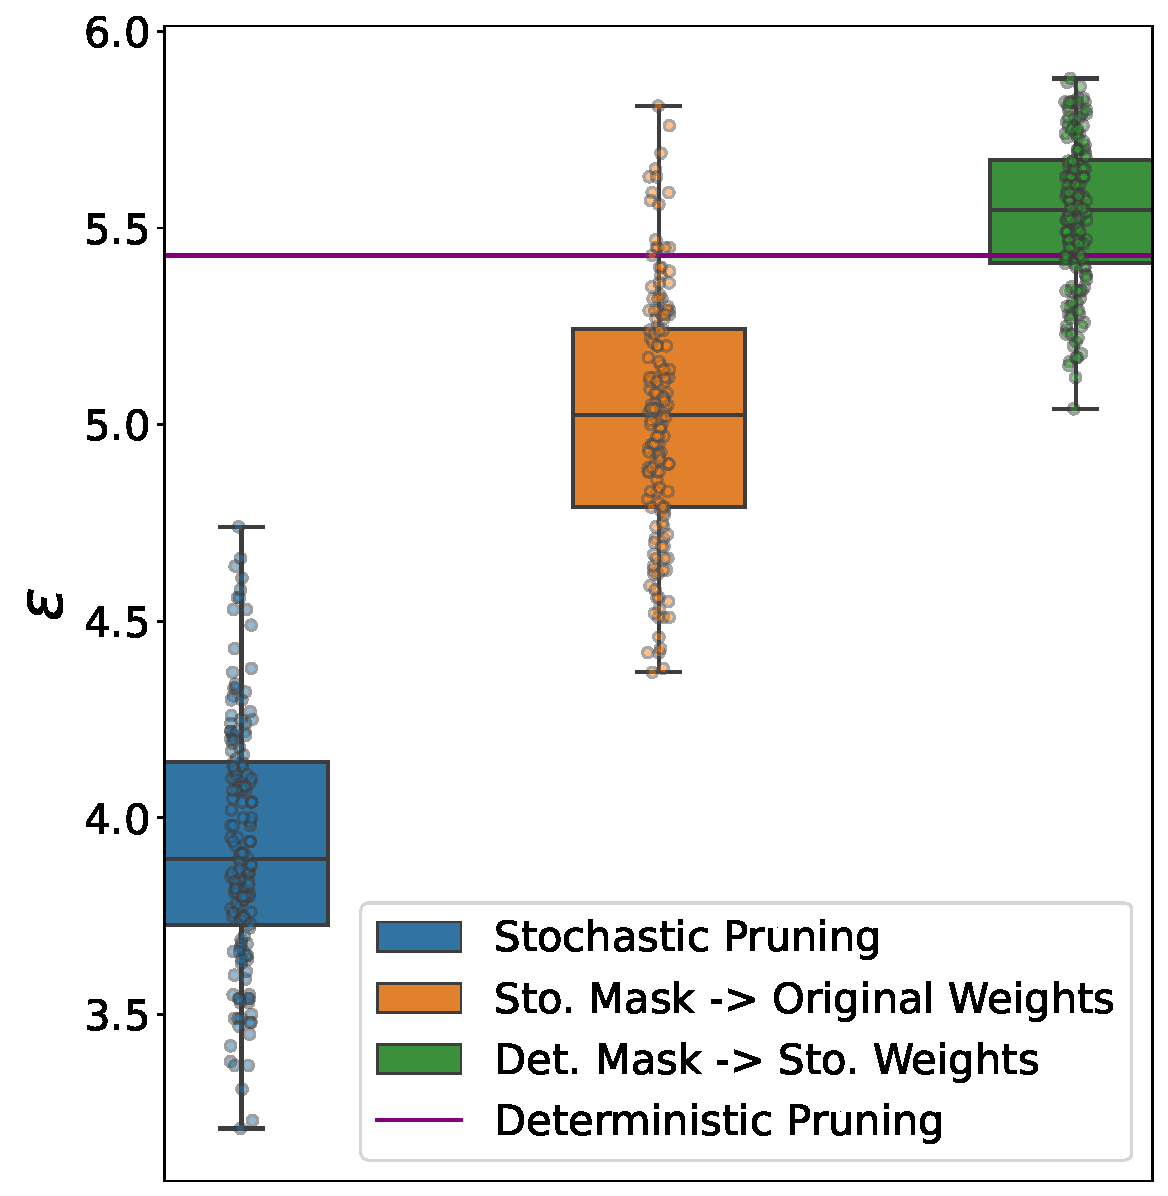
\includegraphics[width=\columnwidth]{figures/epsilon_allN_all_pr_0.8_sigma=0.001.pdf}
   
    \caption{ Pruning rate 0.8} 
    \label{fig:pr0.8sigma0.001}
     \end{subfigure}
    \hfill
     \begin{subfigure}[b]{0.65\columnwidth}
         \centering
     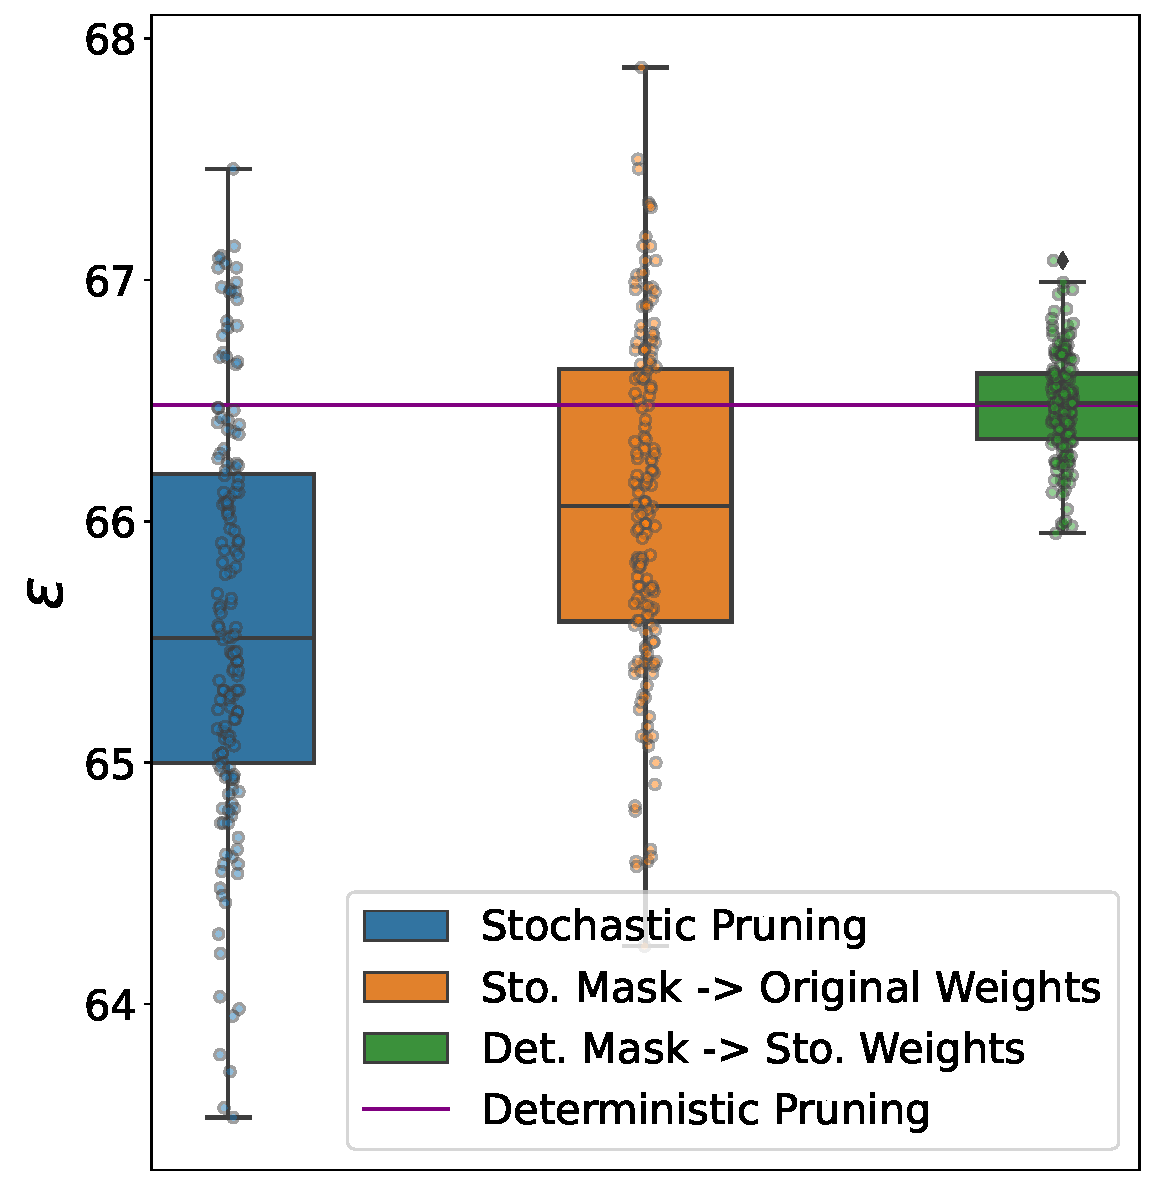
\includegraphics[width=\columnwidth]{figures/epsilon_allN_all_pr_0.9_sigma=0.001.pdf}
    % \caption{Accuracy degradation of One-shot Stochastic Pruning with $\sigma=0.001$ and pruning rate of 0.9} 
    \caption{ Pruning rate 0.9} 
    \label{fig:pr0.9sigma0.001}
     \end{subfigure}
     \caption{Accuracy degradation of One-shot Stochastic Pruning and the resulting models of operations \ref{operation1} and \ref{operation2} with $\sigma=0.001$}
     \label{fig:sigma0.001}
\end{figure*}

\begin{figure*}[!htb]
  \centering
     \begin{subfigure}[b]{0.65\columnwidth}
         \centering
    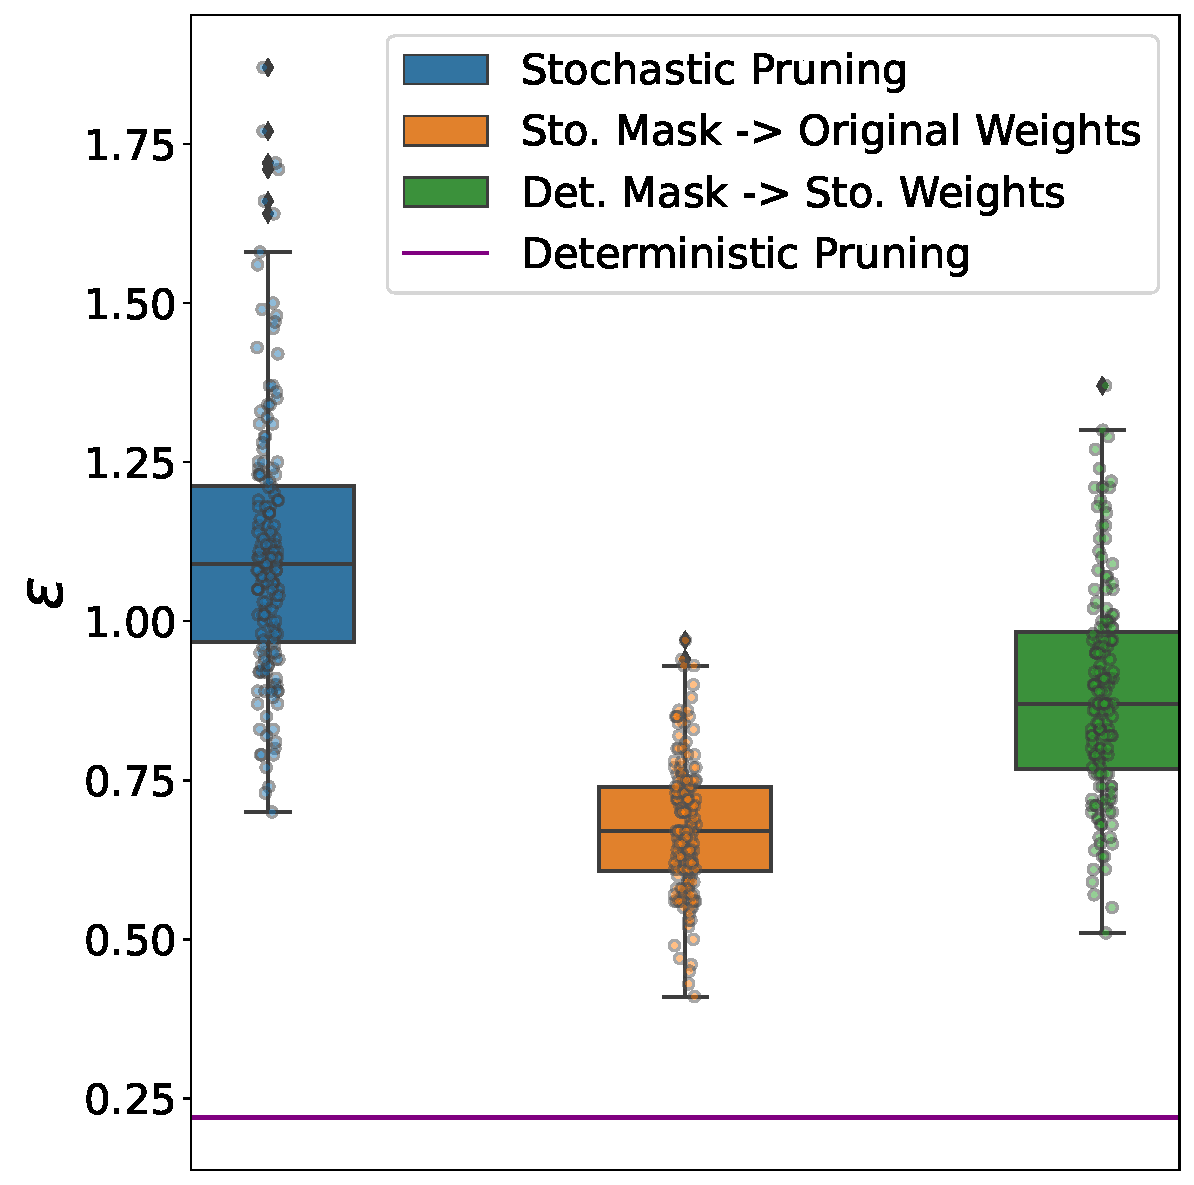
\includegraphics[width=\columnwidth]{figures/epsilon_allN_all_pr_0.5_sigma=0.005.pdf}
    % \caption{Accuracy degradation of One-shot Stochastic Pruning with $\sigma=0.001$ and pruning rate of 0.5} 
    \caption{Pruning rate 0.5} 
    \label{fig:pr0.5sigma0.005}
     \end{subfigure}
     \hfill
     \begin{subfigure}[b]{0.65\columnwidth}
         \centering
   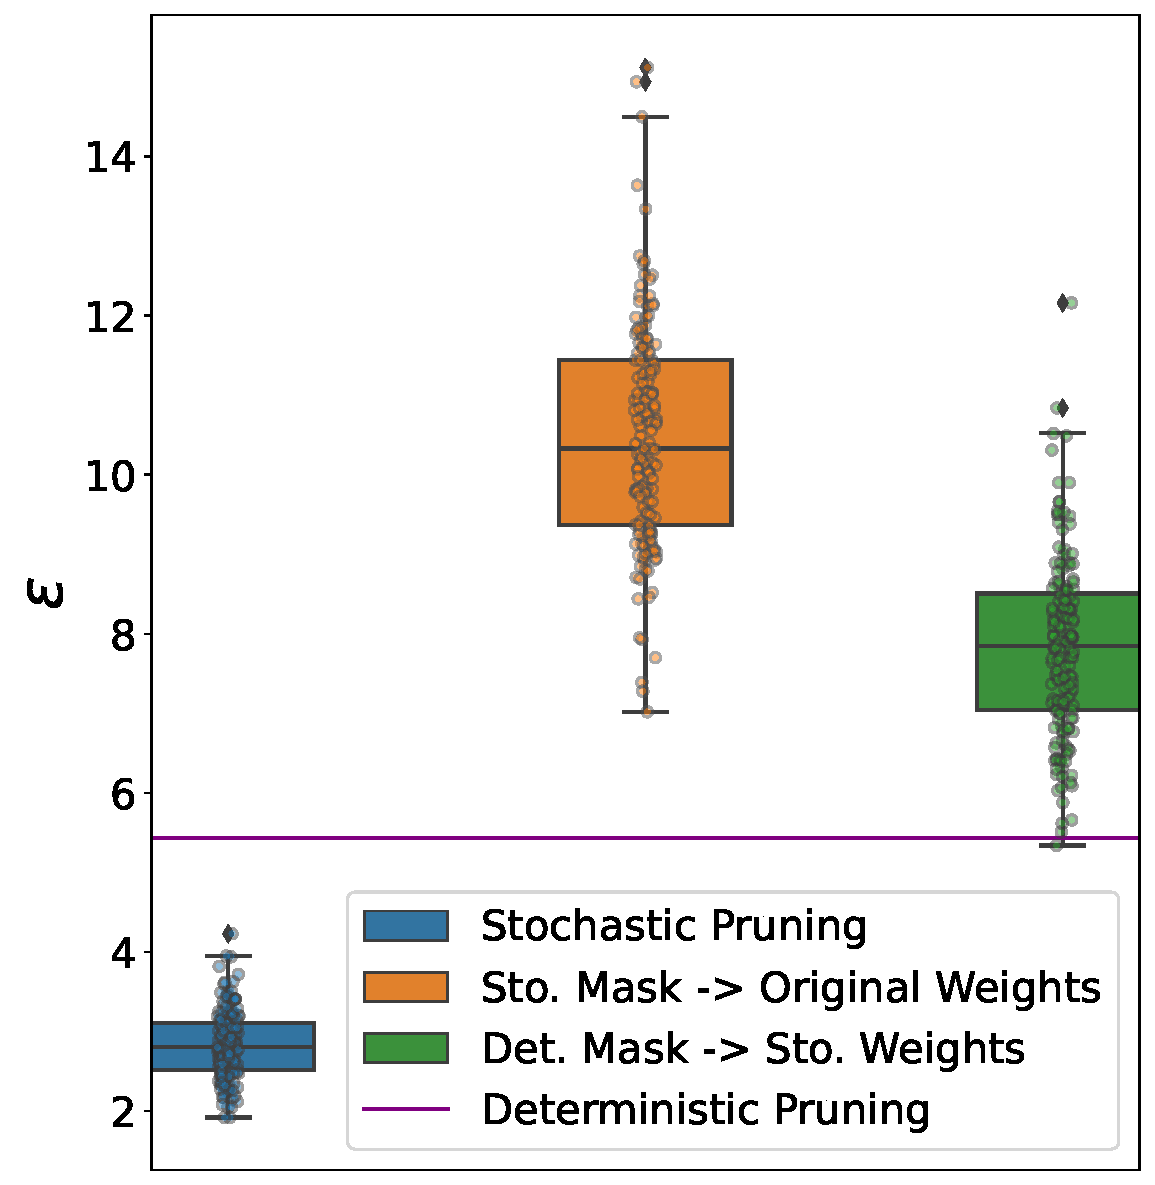
\includegraphics[width=\columnwidth]{figures/epsilon_allN_all_pr_0.8_sigma=0.005.pdf}
   
    \caption{Pruning rate 0.8} 
    \label{fig:pr0.8sigma0.005}
     \end{subfigure}
    \hfill
     \begin{subfigure}[b]{0.65\columnwidth}
         \centering
     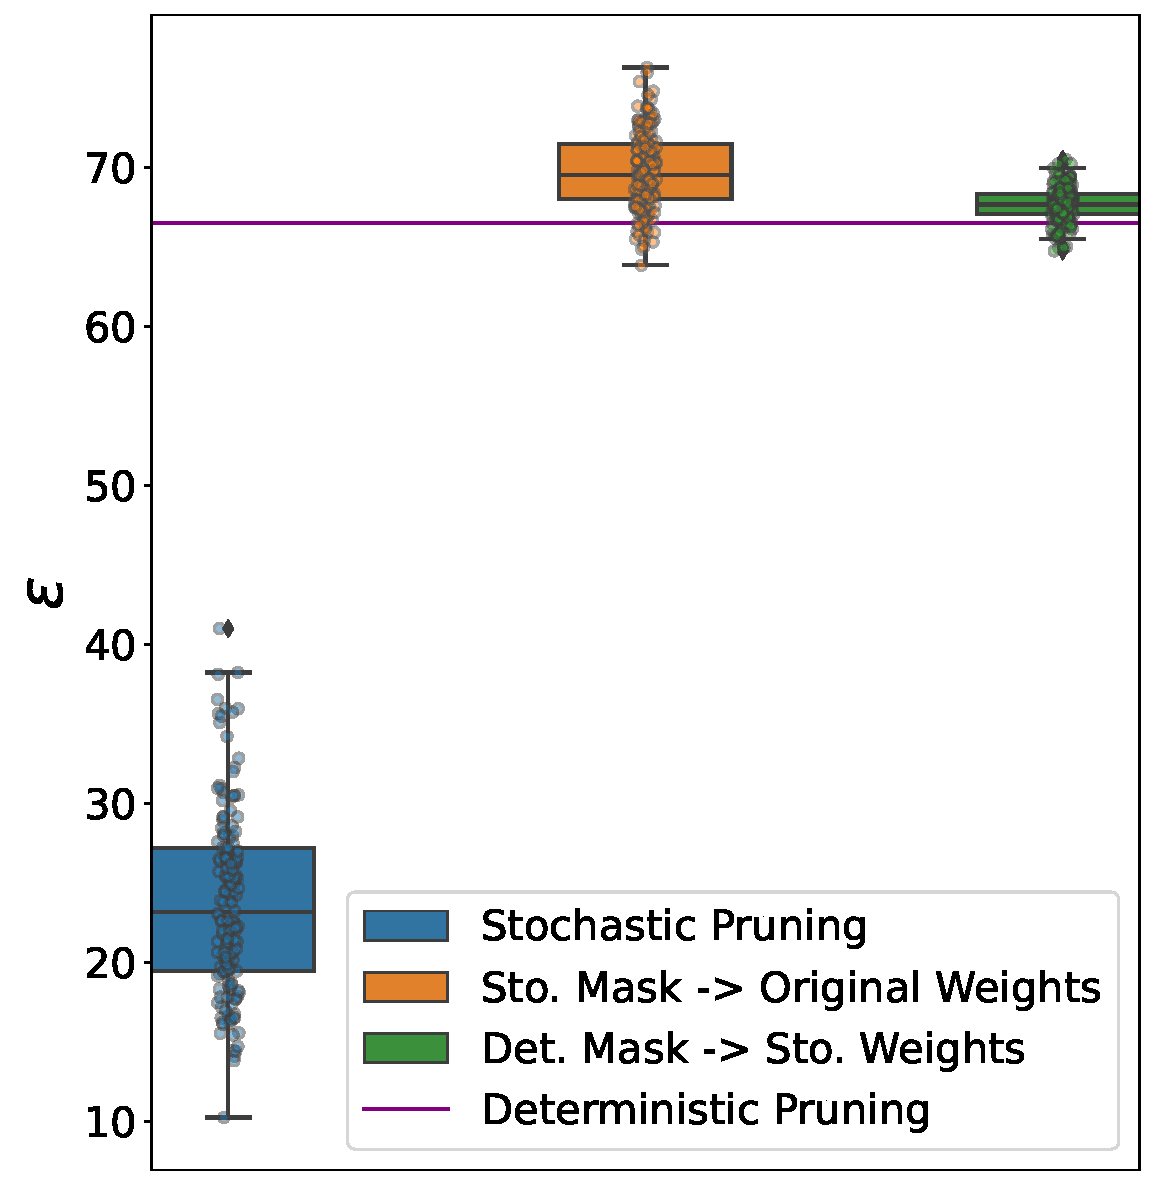
\includegraphics[width=\columnwidth]{figures/epsilon_allN_all_pr_0.9_sigma=0.005.pdf}
    % \caption{Accuracy degradation of One-shot Stochastic Pruning with $\sigma=0.001$ and pruning rate of 0.9} 
    \caption{Pruning rate 0.9} 
    \label{fig:pr0.9sigma0.005}
     \end{subfigure}
     \caption{Accuracy degradation of one-shot Stochastic Pruning and the resulting models of operations \ref{operation1} and \ref{operation2} with $\sigma=0.005$}
     \label{fig:sigma0.005}
\end{figure*}


In \cref{fig:stochastic_versus_deterministic} we observe that this simple operation, which we call \textit{Stochastic Pruning}, produces newly pruned networks that outperform the deterministic pruning of the original network in a one-shot scenario. 

%In \cref{fig:stochastic_versus_deterministic} we see how this simple operation in a one-shot manner already perform better than vanilla deterministic pruning. 
Inspired by \cite{zhouDeconstructingLotteryTickets2019}, where the authors claim that masking can be interpreted as a training procedure, we wanted to know if these newly discovered networks were better due to new weights or because they discovered better masks through \textit{Stochastic pruning}.
To measure this, we performed the following two operations.
\begin{enumerate}[label={\bfseries OP\arabic*}]
    \item We transfer the mask from noisy sparse models (pruned by our) to the original noiseless weights\label{operation1}
    \item We transfer the mask from the deterministic case to noisy weights. \label{operation2}
\end{enumerate}
If operation \ref{operation1} produces better models than deterministic pruning, it means that \textit{Stochastic Pruning} is capable of unveiling good masks and if operation \ref{operation2} produces better models than deterministic pruning, it means that the weights discovered by \textit{Stochastic Pruning}
%\todo{Should I mention stochastic pruning with italics and upper case every time or should I write it like that the first time an later just italics?}
are better than the original weights. In \cref{fig:pr0.8sigma0.001,fig:pr0.9sigma0.001,fig:pr0.8sigma0.005,fig:pr0.9sigma0.005} is the comparison of the accuracy degradation ($\epsilon$) for 160 noisy models for both operations for pruning rates of 0.8 and 0.9. Two main points can be concluded from these results; 1) \textit{Stochastic Pruning} can reveal a better mask for the original weights, but it is greatly affected by the pruning rate and noise level. 
Second, the deterministic mask combined with the noisy weights does not outperform the deterministic pruning of the original model for high levels of pruning. And finally, stochastic weights paired with the mask induced by magnitude pruning can reliably outperform deterministic pruning in the one-shot scenario. Note that the noise only reveals good subnetworks, since none of the dense stochastic networks outperforms the original dense network.


\begin{algorithm}[!tb]
   \caption{Population Based Stochastic Pruning}
   \label{alg:PBRP}
   \begin{algorithmic}[1]
    \STATE {\bfseries Input:} Data $\mathcal{D} $, Trained Weights $w^*$, Maximum number of generations $G$, Population $N$
    \STATE {\bfseries Initialize:} $w_r \gets w^*$,$p_r \gets 0$ 
    \STATE\COMMENT{Our reference model
is initialized to the original model}
   \FOR{$i=1$ {\bfseries to} $G$}
   \STATE $w^*_g \gets$ Null
   %\STATE \COMMENT{Best model for the generation}
   \STATE $p^*_{g} \gets0$ 
   %\STATE \COMMENT{Best generations performance}
   \FOR{ j=1  {\bfseries to} $N$}
   \STATE $w_j \gets w_r+ \mathcal{N}(0,\sigma)$ \COMMENT{Add noise with
   different amplitude per layer}
   \STATE $m_j \gets$ MagnitudePruning($w_j$)
   \STATE $p_j \gets$ Accuracy$(m_j\odot w_j,\mathcal{D})$
   \IF{$p_j>p^*_g$}% \COMMENT{Select the best individual of this generation}

   \STATE $p^*_g\gets p_j$
   \STATE $w^*_g \gets w_j$
   \ENDIF
   \ENDFOR
   \IF{$p_g^* > p_r$}
   \STATE $p_r \gets p^*_g$
   \STATE $w_r \gets w^*_g$
   \ENDIF
   \ENDFOR
   \OUTPUT $w_r$
\end{algorithmic}
\end{algorithm}

\subsection{Population Based Stochastic Pruning}
With this observation, we propose an iterative population-based algorithm that does not use fine-tuning for performance recovery. Our method is simple and more efficient than fine-tuning.
It is known that the distribution of the pruning rate per layer plays a significant role in the performance of sparse networks
\cite{leeLayeradaptiveSparsityMagnitudebased2022}. In this paper we use  the Erdös-Renyí-kernel distribution \cite{evciRiggingLotteryMaking2020} that has been proven to perform well in the random pruning regime \cite{liuUnreasonableEffectivenessRandom2022}. We prune each layer independently from each other.

\textbf{Noise level per layer:}
Since the statistics per layer differ from each other, we decided to use a different noise level ($\sigma$) for each one of them. In \cref{tab:Q50perLayer} are listed the medians of each layer. We decided to set the level of noise to the 10th percentile of the weight magnitude for each layer since we want to affect every layer uniformly.
In \cref{fig:ValidationAccuracy} is depicted \cref{alg:PBRP} applied to a
trained ResNet18 and used the validation set as $\mathcal{D}$. The final
accuracy in the test set for the final weights is 75.6 proving that our method
generalizes.



\begin{figure}[htpb]
    \centering
    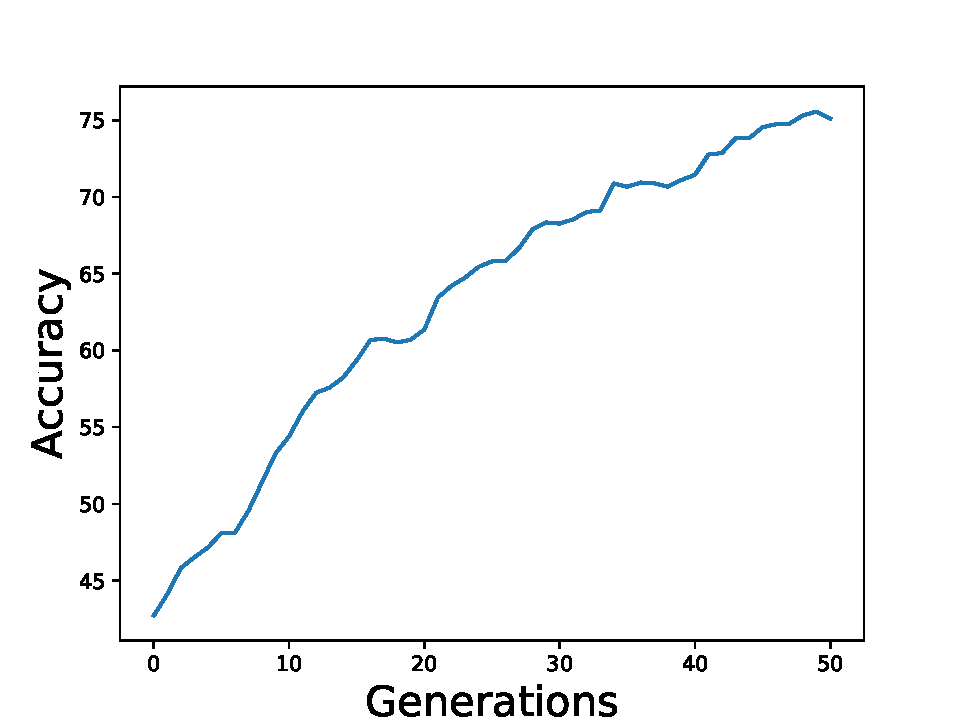
\includegraphics[width=\columnwidth]{val_acc_plot.pdf}
    \caption{Population Based Stochastic pruning results on Validation set for
    CIFAR10 with ResNet18 }
    \label{fig:ValidationAccuracy}
\end{figure}

%\begin{table}[htpb]
%    \centering
%    \caption{Results of PBRP}
%    \label{tab:label}
%    \begin{tabular}{c|c}
%    & \\
%    \end{tabular}
%\end{table}







 
% We performed One-shot \textit{Stochastic Pruning} 160 times on an trained ResNet18 on CIFAR10 and transfer ed the stochastic mask into the original weights



%%%%%%%%%%%% In thi part I talk about how in this images for high pruning rates it seems that the combination of the stochastic weights is  better than the 

% In \cref{fig:OS0.001,fig:OS0.003,fig:OS0.005} can be seen the degradation in accuracy


% I wanted to know if these newly discovered networks were better due to new weights or whether they were better because better masks were found throughout the process.. For this,



% We were interested to know if this procedure was successful.



 % \missingfigure{This is a place holder figure}
%   This figure is to show that for one sample of one-shot pruning we can
%   outperform deterministic pruning for pruning rate 0.8
% \begin{figure}[htb]
%     \centering
%     \includegraphics[width=0.5\textwidth]
%     {transfers_comparison_gaussian_sigma_0.0021419609859022197_pr_0.8_batchSize_512_pop_10_t_14-29.pdf}
%     \caption{}
%     \label{fig:}
% \end{figure}\todo[inline]{Take the title away from ALL THE FIGURES}


  % \begin{figure}[htb]
  %   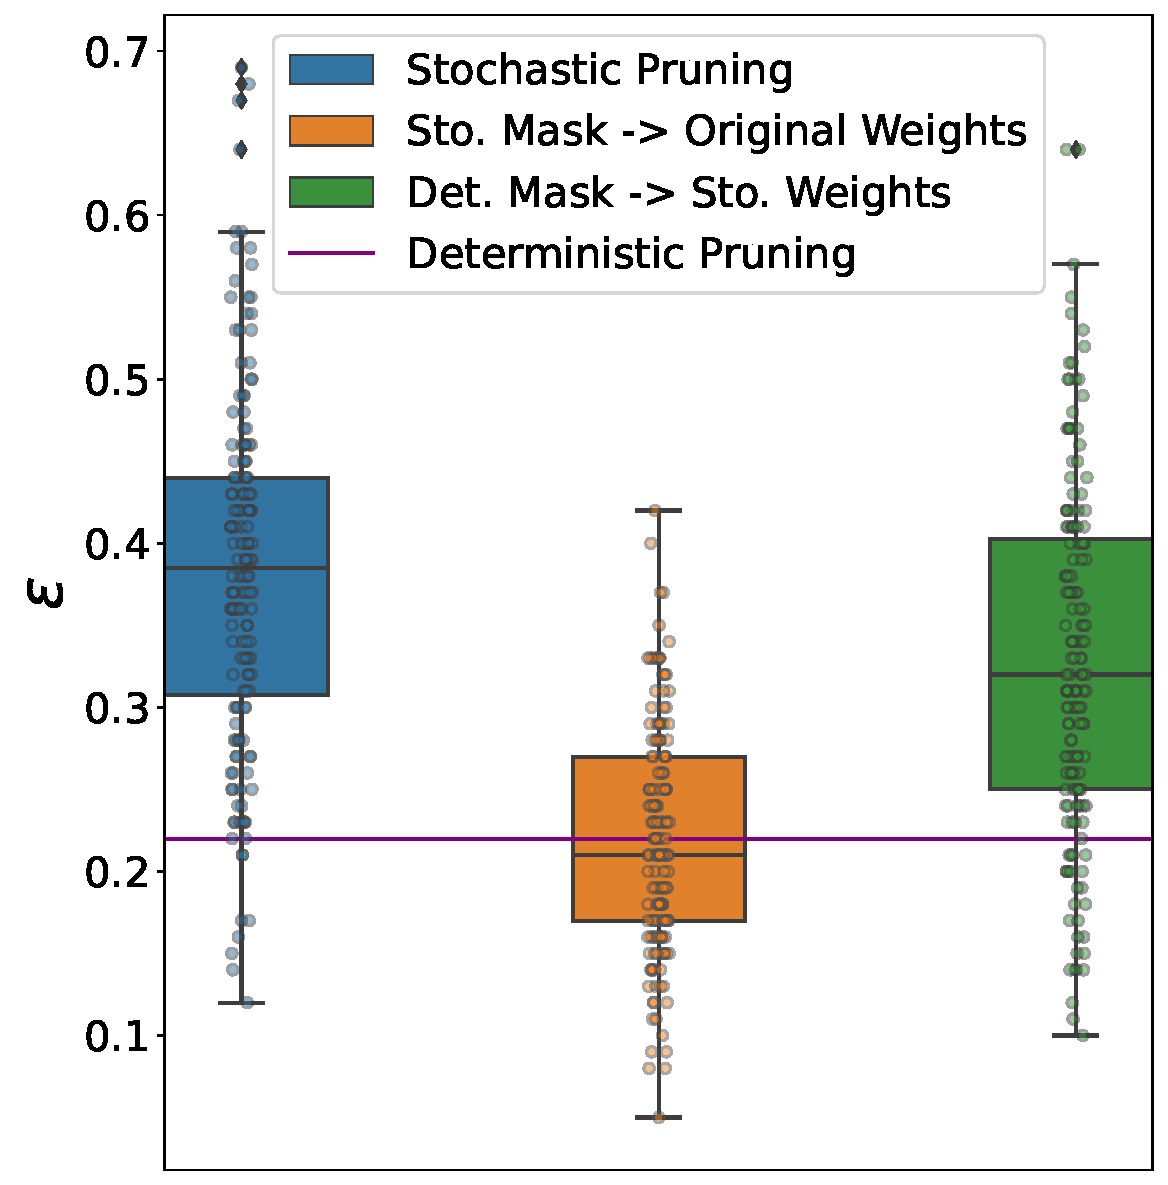
\includegraphics[width=\columnwidth]{figures/epsilon_allN_all_pr_0.5_sigma=0.003.pdf}
  %   \caption{Accuracy degradation on CIFAR10 for one-shot Stochastic Pruning with $\sigma=0.003$ and pruning rate of 0.5} \label{fig:pr0.5sigma0.003}
  % \end{figure}%
  % \begin{figure}[htb]
  %   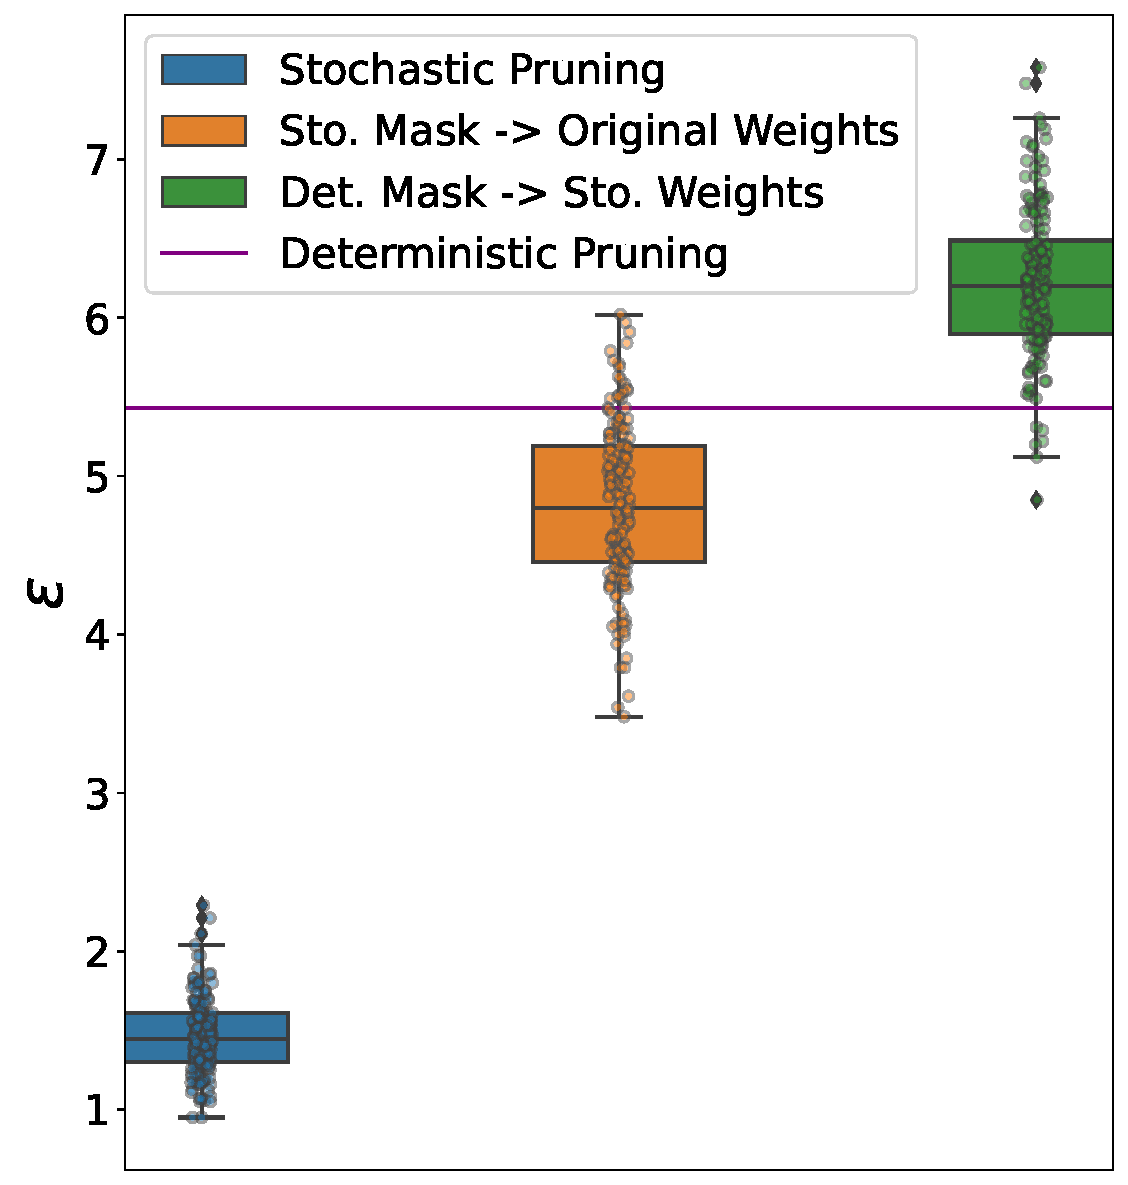
\includegraphics[width=\columnwidth]{figures/epsilon_allN_all_pr_0.8_sigma=0.003.pdf}
  %   \caption{Accuracy degradation on CIFAR10 for one-shot Stochastic Pruning with $\sigma=0.003$ and pruning rate of 0.8} \label{fig:pr0.8sigma0.003}
  % \end{figure}%
  % \hspace*{\fill}   % maximizeseparation between the subfigures
  % \begin{figure}[htb]
  %   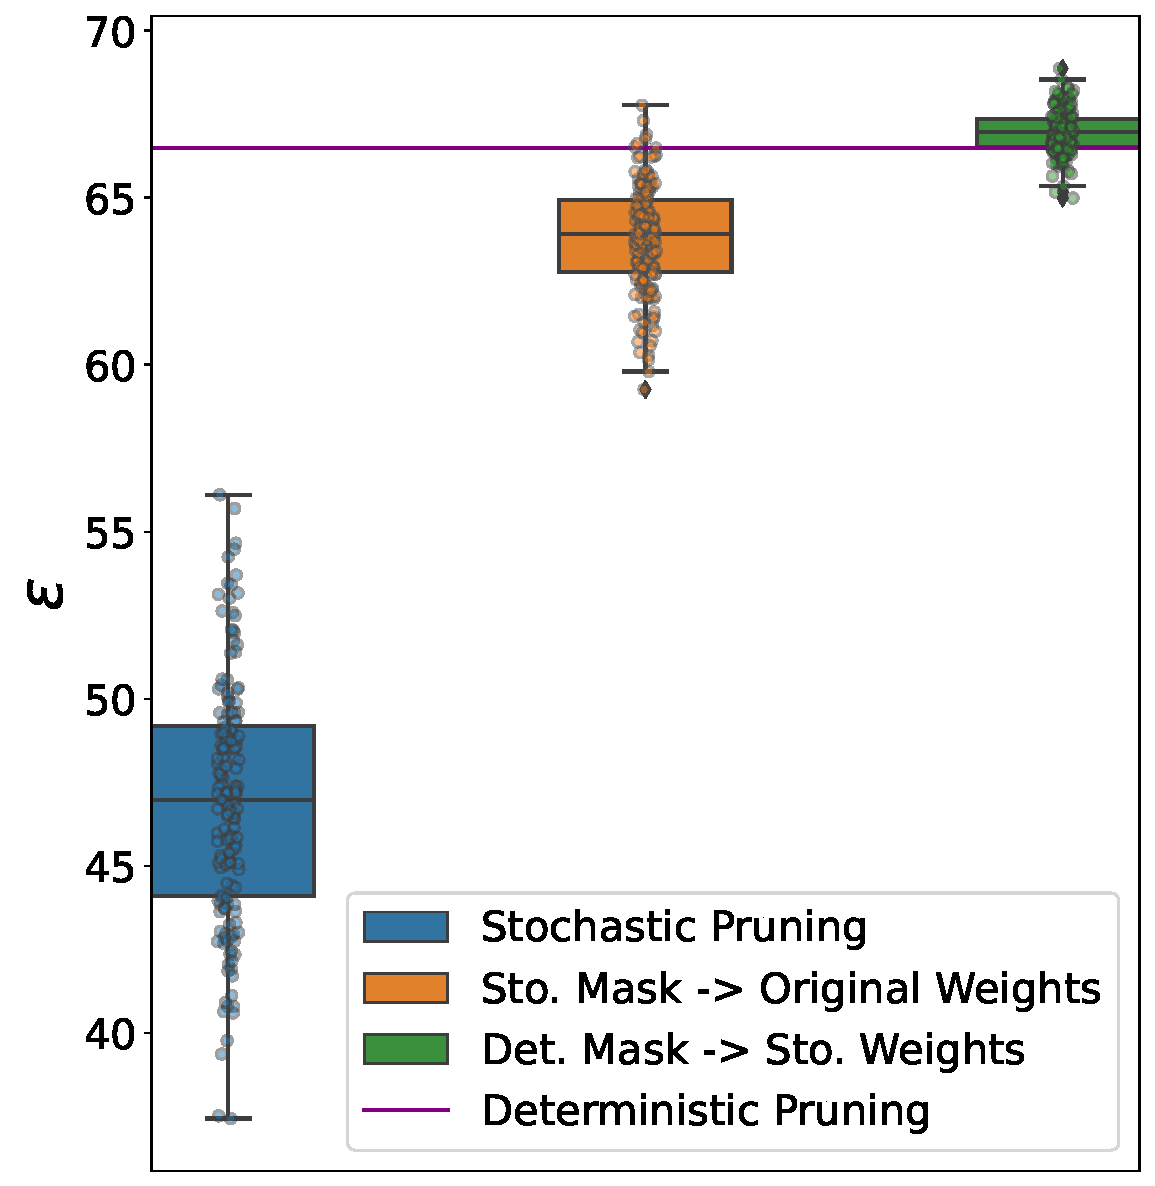
\includegraphics[width=\columnwidth]{figures/epsilon_allN_all_pr_0.9_sigma=0.003.pdf}
  %   \caption{Accuracy degradation of Stochastic Pruning wit $\sigma=0.003$ and pruning rate of 0.9} \label{fig:pr0.9sigma0.003}
  % \end{figure}














  
% \begin{figure}[htb]
%     \centering
%     \includegraphics[width=0.55\textwidth]{}
%     \caption{Accuracy degradation for one-shot stochastic pruning $\sigma=0.005$}
%     \label{fig:OS0.005}
% \end{figure}
  %\begin{figure}[ht]
  %    \centering
  %    \includegraphics[width=\columnwidth]
  %    {epsilon_allN_all_pr_sigma=0.001.png}
  %    \caption{Epsilon for $\sigma=0.001$ varying population size and different
  %    pruning rates}
  %    \label{fig:allNS0.001}
  %\end{figure}
  %\begin{figure}[ht]
  %    \centering
  %    \includegraphics[width=\columnwidth]
  %    {epsilon_allN_all_pr_sigma=0.003.png}
  %    \caption{Epsilon for $\sigma=0.003$ varying population size and different
  %    pruning rates}
  %    \label{fig:allNS0.003}
  %\end{figure}
  %\begin{figure}[ht]
  %    \centering
  %    \includegraphics[width=\columnwidth]
  %    {epsilon_allN_all_pr_sigma=0.005.png}
  %    \caption{Epsilon for $\sigma=0.005$ varying population size and different
  %    pruning rates}
  %    \label{fig:allNS0.005}
  %\end{figure}
